\section{Contribution}

\subsection{Visualization framework}

One of the main issues that had to be dealt with at the beginning of the development process was the issue of how to integrate the visualizations into the ProB 2.0 API. At the time, the software already contained a functioning web server using Java servlets. Since the visualizations are written using Javascript and the d3 Javascript library, they needed to use the same framework. Because the visualizations needed to react to changes that take place during the animation of a model, they needed to be able to communicate with the ProB kernel. In order to accomplish this, a javascript function is invoked when the HTML page is loaded. This javascript sets up an interval so that the servlet that is responsible for the visualization is polled every 300 milliseconds to see if there are any changes. Both the servlet and the javascript function keep track of a counter that functions as a time stamp. This number is sent back and forth. If the javascript function identifies a discrepency between the numbers, it polls the servlet and then updates the visualization.

A problem quickly arose because the servlet is a singleton object. There is only one servlet responsible for all of the visualizations of a particular type. The solution for this was to generate a unique session id for every visualization. Using this id, HTML content for the visualization is generated. When the HTML content is loaded, it calls the correct javascript function which sets up the polling interval and generates the visualization for the calculated data.

Once I implemented a way to integrate the visualization servlets into the ProB 2.0 application, it was still necessary to implement an easy way for the user to interact with the visualizations. One of the main advantages of the D3 visualization framework is the flexibility for the user. Using the D3 selectors, it is possible for the user to select and change the attributes of any of the elements of the visualization. In order to offer this functionality to the users from within the ProB 2.0 application, we decided that we needed to lift the functionality from the javascript level into the existing groovy console in the Java 2.0 API. This was accomplished by creating a \texttt{Selection} object that represents the action that the user wants to carry out in the visualization. Then the \texttt{Selection} object is added to the particular visualization and is applied the next time the visualization is redrawn. The \texttt{Selection} object was written so that its functionality is similar to what the user would actually write using the D3 library.

\begin{verbatim}
\\In the Groovy Console:
\\Define an object to tell the visualization to select the 
\\ circles with ids #croot and #c1 and color them pink
x = viz.selectAll("#croot,#c1").attr("fill","#f36")

\\Add this selection to the visualization with session id "0"
viz.addToSession("0",x)
\end{verbatim}

\subsection{Visualization of the State Space}

During the preliminary experiments for State Space visualization, several different graph libraries were tested out. D3 was chosen because it could process graphs of relatively large size in a way that was eye pleasing for users. Visualization of the state space uses the Spring layout that is available from the D3 library. Unfortunately, when visualizing state spaces with a very large amount of states and inputting them all at the default intitial position, it took rather long for a good visualization to emerge. Therefore, the FRLayout from the JUNG graph library was used as a static rendering engine to calculate the ideal initial positions for the states to be visualized in the graph.

One of the main problems with the web framework that was discovered at the start of the development process was the problem of how different state spaces should be visualized at the same time. The ProB 2.0 API supports the animation of multiple state spaces at any given time. When a state space visualization is created, it is created using the state space that is currently being animated. When the animation is switched, a new state space visualization can be created using the new state space that is being animated. The problem is that a state space visualization is not static. Since the state space that is being visualized changes over time when states are added into the graph, the visualization also needs to adapt and grow correspondingly. The solution to this is to have the instance of the state space visualization poll the state space regularly to get any new states that have been discovered. The problem occured because the servlet responsible for dealing with the state space was static. When the polling occured, the servlet did not know which instance of the state space was supposed to be polled.


(NOT YET IMPLEMENTED)
(ONCE IMPLEMENTED DESCRIBE THE DETAILS OF HOW IT IS IMPLEMENTED)
The visualization of the state space is interactive. The user can grab the nodes within the state space and move them around so that they appear exactly as the user desires. Because it the whole visualization is completely written in d3 and Javascript, it is also possible for the user to dynamically change the DOM of the model using the method described in the above section. It is difficult to create a useful visualization of the whole state space because the user not only wants to inspect how the state space appears as a whole but also the individual states within the operation. Using the zoom functionality available in D3, it was possible to take care of both these needs. The main problem was that if the visualization of the nodes was large enough for the user to read the values of the variable at the given state, it would no longer be easy to see the state space as a whole. This was solved by making the text of the node and edge objects very small. If the user wants to inspect a particular node, they can do so by zooming into the visualization. The text is then larger, and the user only needs to see the nodes that are in the direct neighborhood of the node in question. The user can also click on the background of the visualization in order to p(NOT YET IMPLEMENTED)
(ONCE IMPLEMENTED DESCRIBE THE DETAILS OF HOW IT IS IMPLEMENTED)an and view the other nodes. 

The user can also input Classical B formulas and thereby filter the graph. This uses the algorithms described in \cite{LeTu05_8}. The formula is applied to the state space and all states are merged for which the formula evaluates to the same result. The result is a smaller state space that can be viewed by the user.

\subsection{Visualization of the Value of a Formula Over Time}

During animation in the ProB 2.0 API, the animation steps that have been taken are saved in a trace. A particular formula can take on different values over the course of a trace. In the implementation of the B state space, a particular state is determined by the different values that a variable takes on. Therefore it is particularly interesting to be able to examine the value of a variable over the course of a trace when dealing with a Classical B or Event B formula. 
Evaluation of a formula for takes place in the ProB prolog core. In the ProB 2.0 API, a feature was implemented that takes the list of all the states that the trace covers and a particular formula and returns the list of the values that the formula takes on in the course of the trace. This feature was used in order to create a line plot of the values that the formula takes on. This works for all formulas that take on either an integer value or a boolean value (IMPLEMENT BOOLEAN VALUE).

\subsection{Visualization of a formula}

The ProB CLI already supported the functionality of expanding a formula into its subformulas and finding its value at a given state. However, this functionality would only return the subformulas that were directly beneath the desired formula. For the visualization, it was desired that a given formula could be completely expanded and evaluated and then sent to the ProB 2.0 API. This would ensure that performance would not become an issue. It is now possible to register a Classical B formula in the core and then access the expanded and evaluated formula.

In order to implement the visualization, the d3 tree layout was used \ref{predicate}.

\begin{figure}[ht!]
\centering
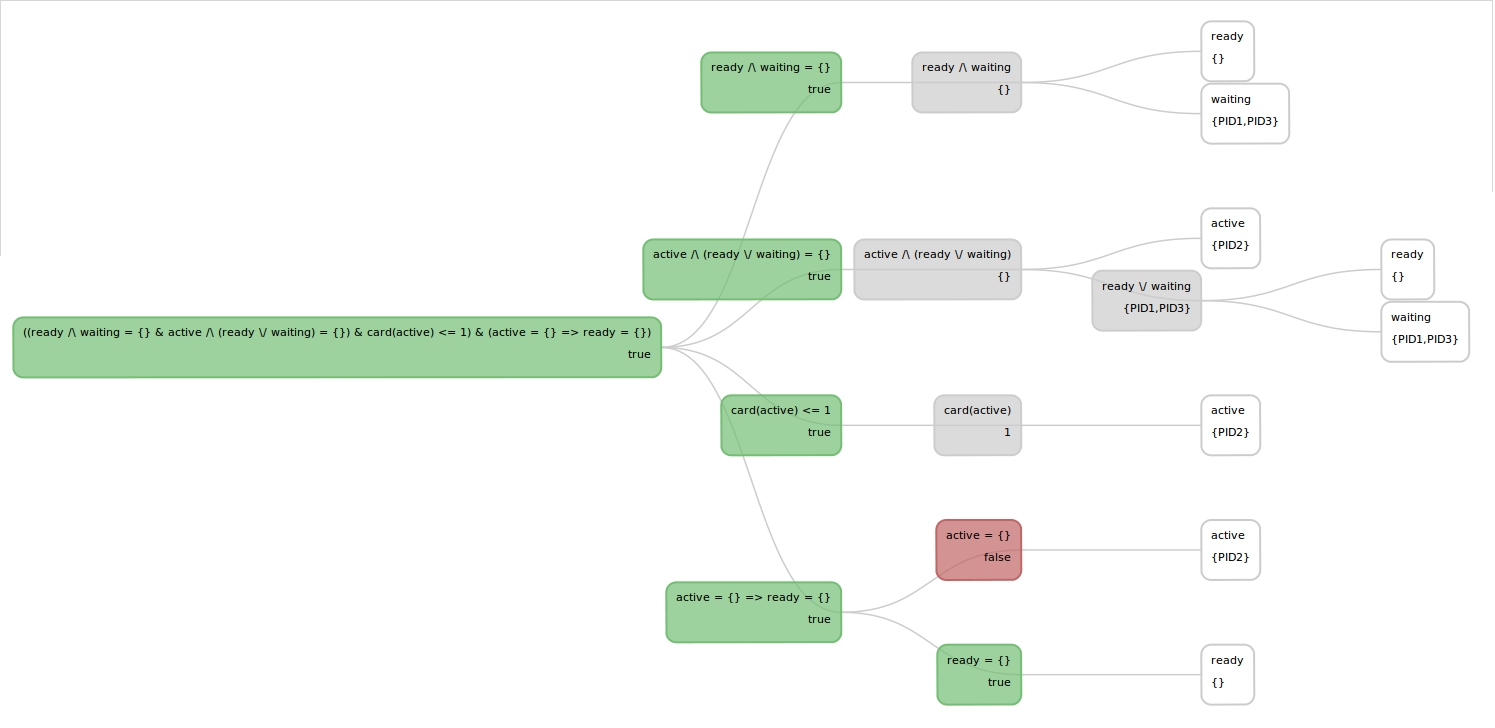
\includegraphics[width=15cm]{bilder/invariant.png}
\caption{Visualization of the invariant of the Scheduler model}
\label{predicate}
\end{figure}

This visualization is interactive. The user can select the nodes to expand or to retract the subformulas. It provides a visualization so that the user can easily interpret the formula. If the formula was evaluated to true for the given formula, the text of the formula is displayed in green. If the formula was evaluated as false, the text is displayed in red. This allows the user to automatically identify the parts of the formula that may have produced the problem. 